\documentclass[10 pt,a4paper]{article}

%% Language and font encodings
\usepackage[brazil]{babel}
\usepackage[utf8x]{inputenc}
\usepackage[T1]{fontenc}
\usepackage[table,xcdraw]{xcolor}

%% Sets page size and margins
\usepackage[a4paper,top=2.5cm,bottom=1.5cm,left=3cm,right=3cm,marginparwidth=1.75cm]{geometry}

%% Useful packages
\usepackage{amsmath}
\usepackage{graphicx}
\usepackage{subcaption}
\usepackage[colorinlistoftodos]{todonotes}
\usepackage[colorlinks=true, allcolors=blue]{hyperref}
\usepackage{url}
\usepackage{natbib}
\usepackage{booktabs}
\usepackage{float}
\usepackage{hyperref}


\title{IF680 - Processamento Gráfico}
\author{Victor Hugo de Lima Kunst}

\begin{document}
\maketitle
\section*{Introdução}
De forma simplificada, esta disciplina se encarrega de introduzir a gráficos e imagens no computador, além de algumas interfaces de entrada e saída.
\linebreak
Está inserida na área da computação que se liga diretamente à visão, sendo esta grande área a qual insere, entre outras, as cadeiras de:
\begin{itemize}
\item Computação gráfica;
\item Processamento gráfico;
\item Visão computacional.
(\cite{sitePet})
\end{itemize}


\section*{Relevância}
De acordo com \textit{Computer Graphics - Priciples and Practice}, de James D. Foley \cite{ComputacaoGrafica}, "The most striking aspect of graphics in our everyday lives is the 3D imagery being used in video games and special effects in the entertainment industry and advertisements. But our day-to-day interactions with home computers, cell phones, etc., are also based on computer graphics", ou seja, embora a parte mais impressionante dos gráficos em nossas vidas seja a imagem 3D sendo utilizada em videogames (figura \ref{figura1}) e em efeitos especiais na indústria de entretenimento e propaganda, nossa interação diária com computadores, celulares, entre outros (figura \ref{figura2}), são baseados em gráficos computadorizados. Este e outros exemplos provam a importância do estudo gráfico.\linebreak
Neste segmento, a cadeira em questão tem como um dos seus objetivos a preparação para os fundamentos de computação gráfica:
\begin{itemize}
\item É visto a parte da modelagem geométrica (introdução e desenvolvemento de curvas e superfíceis, criando assim uma teoria, algo próximo de um cálculo, para curvas e superfíceis paramétricas);
\item É introduzido uma parte de visulização, onde o aluno deve gerar um sistema gráfico no qual ele faz todas as funções à mão: De forma mais especifica, a única parte que utilizaria a biblioteca gráfica seria para pintar um pixel de alguma determinada cor, ou seja, toda a parte do cálculo de iluminação e encontrar atributos de cena e textura é feita manualmente;
\item Desta forma o aluno poderá compreender os detalhes e a parte de como funciona, para que depois possa utilizar a biblioteca gráfica com mais clareza.
(\cite{Silvio})
\end{itemize}
Um ponto que poderia se considerar negativo por muitos estudantes nesta cadeira poderá ser a matemática envolvida. Na primeira página do segundo capítulo de \textit{Curves and Surfaces for CAGD - A Practical Guide}, de Gerald Farin \cite{CurvaseSuperficeis}, temos uma comparação de como seria o trabalho de um estilista ou designer sobre um objeto, ou seja de forma não matemática, e de como serão discutidos os objetos no livro. No site da disciplina podemos ter uma ideia de como seria esta parte (\(\text{\cite{siteCadeira}} \rightarrow \text{projetos}\)).
\begin{figure}[H]
 \centering
 \begin{subfigure}[H]{0.25\linewidth}
 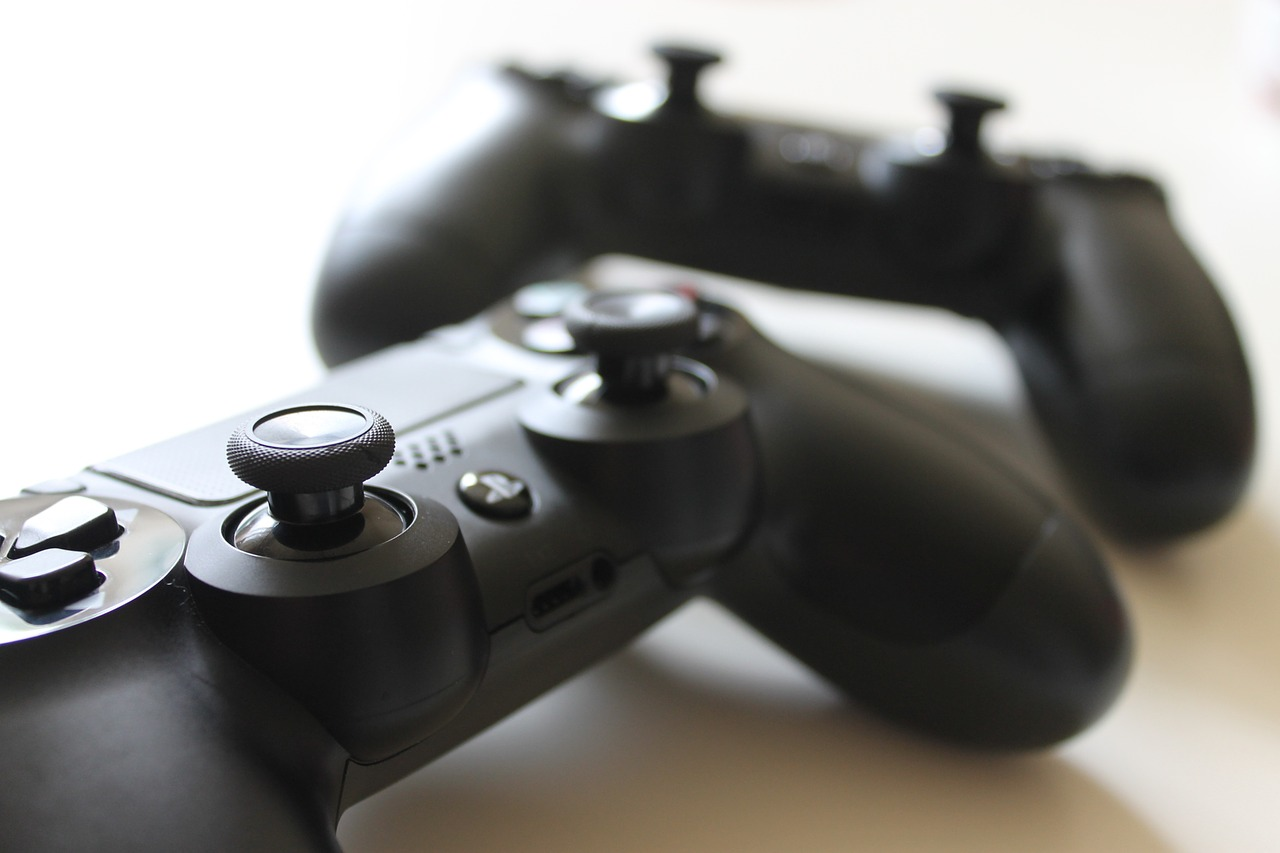
\includegraphics[width=\linewidth]{controle.jpg}
 \caption{videogames e seus gráficos}
 \label{figura1}
 \end{subfigure}
 \begin{subfigure}[H]{0.25\linewidth}
 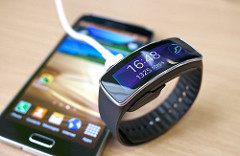
\includegraphics[width=\linewidth]{celular.jpg}
 \caption{vários itens utilizam gráficos computadorizados}
 \label{figura2} 
 \end{subfigure}
\end{figure}
%a figura 1 apresenta CC0, encontrado no link {https://pixabay.com/pt/joystick-console-jogos-de-v%C3%ADdeo-1216816/}
%a figura 2 apresenta CC2, de acordo com o site https://www.flickr.com/photos/janitors/13537777475 e seu autor é Kārlis Dambrāns


\section*{Relações com outras disciplinas}

\begin{table}[H]
\centering
\begin{tabular}{@{}|l p{7cm}|@{}}
\toprule
\multicolumn{1}{|c|}{\textbf{CADEIRAS}}                                                 &\multicolumn{1}{|c|}{\textbf{RELAÇÃO ENTRE SI}}                                                                                                                                                                                                                                                                                                                \\ \midrule
\multicolumn{1}{|c|}{REALIDADE VIRTUAL - IF755} & Na realização de alguns problemas da Realidade Virtual há uma necessidade de utilização de algumas propriedades que envolvem processamento gráfico.                                                                                                                                                                                                            \\ \midrule
\multicolumn{1}{|c|}{COMPUTAÇÃO GRÁFICA - IF750}                                               & Processamento Gráfico pode ser visto como uma introdução à Computação Gráfica, como já foi visto acima.                                                                                                                                                                                                                                                        \\ \midrule
\multicolumn{1}{|c|}{INTERFACES GRÁFICAS - IF865}                                              & Como o nome já sugere, Interfaces Gráficas necessita de uma base na parte gráfica, o que inclui assuntos vistos em Processamento Gráfico.                                                                                                                                                                                                                      \\ \midrule
\multicolumn{1}{|c|}{PROJETO IMPLEMENTAÇÃO JOGOS 2D - IF793}                                   & É essencial uma base em gráfico para implementação de jogos no geral.                                                                                                                                                                                                                                                                                          \\ \midrule
\multicolumn{1}{|c|}{TÓPICOS AVANÇADOS EM MÍDIAS - IF760}                                      & Por trabalhar na área de Human-Robot Interaction (HRI), é interessante uma base prévia em gráficos para que possa "identificar estratégias inovadoras e métodos eficientes utilizados para este tipo de interação pela comunidade científica".                                                                                                                 \\ \midrule
\multicolumn{1}{|c|}{INTRODUÇÃO A MULTIMÍDIA - IF687}                                          & Para que possa criar seus ''mundos virtuais'' é imprescindível uma base em gráficos, que começa pela cadeira de Processamento Gráfico.                                                                                                                                                                                                                           \\ \midrule
\multicolumn{1}{|c|}{VISÃO COMPUTACIONAL - IF752}                                              & Como envolve a modelação computacional de aspectos da visão humana, é importante ter uma base sólida em Processamento Gráfico para realizar suas atividades. Todas as cadeiras que estão dentro de uma mesma área da computação devem, deveras, ter alguma relação entre si, como é o caso de Processamento Gráfico, Computação Gráfica e Visão Computacional, que estão na área que lida com a parte diretamente ligada à imagem (visão). \\ \bottomrule 
\end{tabular}
\linebreak
\linebreak
\end{table}

\bibliographystyle{alpha}
\bibliography{sample}

\end{document}